\section{Constructing Parallelisations}
In order to first motivate some of the results in this section, we will prove the famous Hairy Ball Theorem\footnote{Depending on the referece, this theorem may either refer to the case of all even dimensional spheres or simply the case for $\mathbb{S}^2$ - in this case we will opt for the latter characterisation.}. We will see that this is in fact a special case of a more general theorem which we will also prove. Two proofs are given, one of an analytic nature due to Milnor \cite{MR505523} and the other using the Poincar\`{e}-Hopf theorem which we prove.
We shall then construct explicit parallelisations for $\mathbb{S}^n$, $n=1,3,7$. Finally we discuss results related to the existence of division algebras.
 
\begin{proposition}
The sphere $\mathbb{S}^2$ does not admit a non-vanishing continuous tangent vector field and hence, $\mathbb{S}^2$ is not parallelisable.
\end{proposition}

%\begin{proof}
%Suppose, for a contradiction, that $\mathbb{S}^2$ does in fact admit a continuous non-vanishing vector field $V$. Since $V$ is non-vanishing we may assume that $V$ has unit length, or else renormalise, $\frac{V}{|V|}$.
%\end{proof}
%
%To prove this, we will prove the Poincar\`{e}-Hopf theorem for surfaces which will immediately imply the result.
%
Before we prove the above proposition, we have the following definitions.

\begin{definition}
A \textit{Riemannian metric} (often referred to simply as a metric; not to be confused with a distance function) $g$ on a smooth manifold $M$ is a smooth choice of inner product on each tangent space of the $M$, $g_x:T_xM\times T_xM\to\mathbb{R}$. Since $g$ is an inner product, for all $x\in M$, $g=g_x$ satisfies the following.
\begin{enumerate}
\item $g(u,v)=g(v,u)$, $\forall u,v\in T_xM$.
\item $g(u,v)\geq 0$, $\forall u\in T_xM$.
\item $g(u,v)=0$ if and only if $u=0$.
\end{enumerate}
Further, $g$ is said to be smooth in the sense that if $X,Y$ are smooth vector fields, then $x\mapsto g_x(X_x,Y_x)$ is smooth.

In local coordinates, a metric can be described in terms of its coefficients in a local chart, given by $g_{ij}=g(\partial_i,\partial_j)$. Smoothness of $g$ is equivalent to smoothness of the coefficient functions $g_{ij}$ is a given chart.
\end{definition}

%\textcolor{red}{\textbf{Connection 1-form}: Bugger, going to have to rethink this...}
\begin{definition}
An atlas $\mathcal{A}$ for a smooth manifold $M$ is \textit{orientable} if whenever charts $\varphi$ and $\eta$ in $\mathcal{A}$ have a non-trivial, common domain of definition, the Jacobian $\det(\eta\circ\varphi^{-1})$ is positive. An \textit{orientation} on an orientable manifold is an equivalence class of oriented atlases, where two oriented atlases are equivalent if their union is an oriented atlas.
\end{definition}
\begin{definition}
The \textit{Euler characteristic}, denoted by $\chi=\chi(M)$ (not to be confused with the space of all vector fields on $M$, though this should be clear from context), is a topological invariant. If $M$ admits a triangulation, (i.e. a decomposition into diffeomorphic images of closed $n$-simplices such that the intersection of any two is either empty or a common $(n-k)$-simplex ($k<n$)), then the Euler characteristic is given by
\[
\chi(M)=\sum_i(-1)^is_i,
\] 
where the $s_i$ are the number of $i$-dimensional simplices of a given triangulation of $M$.
It is a well known, though non-trivial to prove, result that every smooth manifold does admit such a triangulation \cite{whitehead1940c1}. Furthermore, if the manifold is compact then the triangulation may be chosen such that it is finite.
\end{definition}

Now, consider the following results regarding compact oriented two-dimensional manifolds.

\begin{theorem}[Gauss-Bonnet]
Let $M$ be a compact oriented two-dimensional manifold equipped with a Reimannian metric $g$. Let $K$ be the Gaussian curvature of $M$ and $k_g$ be the geodesic curvature of $\partial M$. Then,
\[
\int_MK\,dA+\int_{\partial M}k_g\,ds=2\pi\chi(M).
\] 
\end{theorem}
\begin{proof}
Refer to \cite{andrews} or \cite{guillemin2010differential}.
\end{proof}
\begin{theorem}[Poincar\'{e}-Hopf (Surfaces)]
Let $M$ be a compact oriented two-dimensional manifold. Let $V$ be any vector field on $M$ which has all zeroes isolated, that is, if $y$ is any zero of $V$ then there is a neighbourhood $U$ of $y$ in $M$ such that $V$ is non-zero on $U\backslash\{y\}$. Label the zeroes of $V$ as $x_1,\ldots,x_k$. Then 
\[\sum_{i=1}^{k}\mathrm{Ind}_x(V)=\chi(M).\]
\label{thm:poinhopf}
\end{theorem}
\begin{proof}
A proof of the generalised form of this theorem for manifolds is presented in Section \ref{sec:ph-gen-sec}.
\end{proof}
%The following proof is due to Andrews,\cite{andrews}.
%\begin{proof}
%Let $V$ and $g$ be given and let $x_1,\ldots,x_N$ be the zeroes of $V$. About each zero, choose a neighbourhood $U_i$ of $x_i$ such that $V$ is non-vanishing on $\tilde{M}=M\backslash\bigcup_{i=1}^NU_i$. Let $\gamma_i$ be the boundary of the $U_i$ parametrised anticlockwise in some oriented chart.
%
%Define $e_1=\frac{V}{g(V,V)^{1/2}}$ and take $e_2$ to be the unit vector orthogonal to $e_1$. Denote the dual frame by $\omega_1$ and $\omega_{2}$.
%\textbf{\textcolor{red}{TBC?}}
%\end{proof}
\begin{remark}
We note that since $\mathbb{S}^2$ has no `edge' the integral over $\partial\mathbb{S}^2$ is zero. Furthermore, recall that the Gaussian curvature of $\mathbb{S}^2$ with the standard metric is 1 \cite{andrews}. From Gauss-Bonnet we have that the left-hand side is non-zero and so the right-hand side must be non-zero, i.e. the Euler characteristic is non-zero. It follows by Poincar\`{e}-Hopf that any vector field $V$ on $\mathbb{S}^2$ must vanish somewhere. Thus, $\mathbb{S}^2$ is not parallelisable. 
\end{remark} 
We have the following more general result (which also immediately implies the Hairy Ball Theorem).
\begin{theorem}
\label{thm:novan-iff-odd}
The sphere $\mathbb{S}^n$ admits an everywhere non-zero smooth vector field if and only if $n$ is odd.
\end{theorem}
In order to prove this result, we will break the theorem up into two parts. Proposition \ref{prop:even-noVF} will give the necessary condition and then in Section 3.2 we will provide the sufficient condition for the theorem.
\begin{proposition}
\label{prop:even-noVF}
If $n$ is even, then there exists no nowhere vanishing smooth vector field on $\mathbb{S}^n$.
\end{proposition}
The following proof is due to Milnor \cite{MR505523} and uses only basic techniques from analysis as opposed to other proofs that make use of more algebraic methods such as (co)homology theory.
\begin{proof}
Suppose for the sake of a contradiction, that such a vector field $V:\mathbb{S}^n\to\mathbb{R}^{n+1}$ exists. Without loss of generality, we may set $\|V(x)\|=1$ for all $x$, otherwise we may simply normalise the vector since by hypothesis $\|V(x)\|\neq 0$. Let $A$ be a compact region of $\mathbb{R}^{n+1}$ given by,
\[
A=\{y\in\mathbb{R}^{n+1}:1-\varepsilon\leq\|y\|\leq 1+\varepsilon\},
\] 
for $0<\varepsilon<1$. We can expand $V$ onto $A$ by continuing linearly over the rays, i.e. set $V(x)=\|x\|V(\frac{x}{\|x\|})$. Now consider the function,
\[
f_t(x)=x+tV(x),
\]
for $t\in\mathbb{R}$ and which is defined for all $x\in A$. Furthermore, since $\langle x,V(x)\rangle=0$ for all $x\in A$, we have that $\|f_t(x)\|=\|x\|\sqrt{1+t^2}$.

We now have the following lemmas which will give us the contradiction we seek.
\begin{lemma}
For sufficiently small $t>0$, the mapping $f_t$ is one-to-one and maps the region $A$ onto a region $f_t(A)$ whose volume can be expressed as a polynomial function in $t$.
\end{lemma}
\begin{proof}
Since $A$ is compact and since $V$ is smooth, there exists a Lipschitz constant $c>0$ such that,
\[
\|V(x)-V(y)\|\leq c\|x-y\|,
\]
for all $x,y\in A$. We see this from the fact that since all the partial derivatives are continuous, by the mean value theorem from calculus, they attain a maximum on $A$ and taking the maximum of these yields $c$.

Choose $t$ such that $|t|<c^{-1}$ and suppose that $f_t(x)=f_t(y)$. Then we get $x-y=t(V(y)-V(x))$ and hence \[\|x-y\|=|t|\|V(y)-V(x)\|\leq c|t|\|x-y\|,\] and since $0<|t|c<1$, we have that $x=y$ and so $f_t$ is injective.\\

Via the change of variables theorem, we have that,
\[
\mathrm{vol}(f_t(A))=\int_{f_t(A)}1\,\mathrm{d}y=\int_A|\mathrm{det}(Df_t(x))|\,\mathrm{d}x.
\]
We note that since $Df_t(x)=I+tD\,V(x)$ (where $I$ is the identity matrix) and the determinant of a finite dimensional matrix is a polynomial in its entries, we get that \[\mathrm{det}(Df_t(x))=1+t\sigma_1(x)+\ldots+t^k\sigma_k(x),\] where the $\sigma_i$ are polynomials of all the partial derivatives of $V$ and hence continuous in $x$. Now, choosing $t$ sufficiently small, we have that $\mathrm{det}(Df_t(x))>0$ for all $x\in A$ and we have,
\begin{align*}
\mathrm{vol}(f_t(A))&=\int_A|\mathrm{det}(Df_t(x))|\,\mathrm{d}x\\
&=\int_A\mathrm{det}(Df_t(x))\,\mathrm{d}x\\
&=\int_A\sum_{i=0}^kt^i\sigma_i(x)\,\mathrm{d}x\\
&=\sum_{i=0}^kt^k\left[\int_A\sigma_i(x)\,\mathrm{d}x\right],
\end{align*}
which is clearly a polynomial function in $t$. This completes the proof of the lemma.
\end{proof}
\begin{lemma}
For sufficiently small $t>0$, the unit sphere is mapped onto the sphere of radius $\sqrt{1+t^2}$.
\end{lemma}
\begin{proof}
When $t$ is sufficiently small, such that the determinant of $Df_t(x)$ is always strictly positive and hence $Df_t(x)$ is non-singular, we have via the inverse function theorem that $f_t$ maps open sets to open sets. As such, if we restrict $f_t$ from $\mathbb{S}^n$ to the ball $B^{n+1}$ of radius $\sqrt{1+t^2}$, we have that $f_t(\mathbb{S}^n)$ is open in the larger sphere. On the other hand, since we are working in a finite dimension, $\mathbb{S}^n$ is compact and so we have that the image under $f_t$ is also compact and hence closed in the larger sphere. Since the codomain is connected, we have that the image is both open and closed in the codomain, and so it must be the entire sphere, i.e. $f_t(\mathbb{S}^n)=B^{n+1}_{\sqrt{1+t^2}}$ and the result follows. 
\end{proof}
By the second lemma, we get that $A$ is mapped onto $\{\sqrt{1+t^2}(1-\varepsilon)\leq\|x\|\leq\sqrt{1+t^2}(1+\varepsilon)\}$, which has volume $\sqrt{1+t^2}^{n+1}\mathrm{vol}(A)$. If $n$ is even, then $\sqrt{1+t^2}^{n+1}$ is not a polynomial function. Hence, we get a contradiction with lemma 1 and so our original assumption that there exists a nowhere vanishing smooth vector field on $\mathbb{S}^n$ must be incorrect.
\end{proof}
As we are about to see, this motivating example of the Hairy Ball theorem is merely a special case of the following more general result, which also acts as a stepping stone to establishing which sphere admits parallelisations.\\

\subsection{Existence of a Non-Vanishing Vector Field}
As we have seen in the previous example and theorem, even dimensional spheres do not admit even a single everywhere non-zero smooth vector field. This tells us that we must focus our study solely on odd dimensional spheres. Ultimately, we wish to establish some maximal number of independent vector fields; before this however, an important question to perhaps ask, is whether there exists even one pointwise linearly independent vector field on $\mathbb{S}^n$.

The answer to this question thankfully, is ``yes'', we can guarantee the existence of at least one nowhere vanishing smooth vector field on $\mathbb{S}^n$. If $n$ is odd, writing $n=2k-1$, the sphere $\mathbb{S}^n$ can be embedded in $\mathbb{R}^{2k}$ and we can write down the following nowhere vanishing vector field $V:\mathbb{S}^{2k-1}\to\mathbb{R}^{2k}$ given by,
\begin{equation}
V(x_1,x_2,\ldots,x_{2k-1},x_{2k})=(-x_2,x_1,\ldots,-x_{2k},x_{2k-1}).
\label{eq:novan-vect-1}
\end{equation}
Clearly, any point $x$ on the sphere is not zero and so $V(x)$ is nowhere vanishing for all points $x\in\mathbb{S}^{2k-1}$.\\

Furthermore, we have,
\[
x\in\mathbb{R}^{2k}\mapsto (x,V(x))\in\mathbb{R}^{2k}\times\mathbb{R}^{2k}=T\mathbb{R}^{2k}.
\] 
Consider the position vector field on the sphere $R$ which is given by,
\[
x\mapsto (x,x),
\]
It can be shown through a tedious but simple computation that,
\[
\langle V(x),R(x)\rangle=0.
\]
This is to say then that the vector field $V$ is orthogonal $R$, but $R$ is also the normal vector field to the sphere. So $V$ must be tangent to the sphere.\\

The construction given above together with Proposition \ref{prop:even-noVF} concludes the proof for Theorem \ref{thm:novan-iff-odd}.

\subsection{Poincar\`{e}-Hopf (General) \label{sec:ph-gen-sec}}
\begin{theorem}
Let $M$ be a compact orientable manifold, then there exists a non-vanishing vector field on $M$ if and only if $\chi(M)=0$.
\end{theorem}
We give a sketch of the proof below, many of the proofs of the lemmas stated are omitted. We refer the reader to \cite{wrightPoincare} for details.
\begin{proof}
We must first define the mapping degree of a map between orientable manifolds. Take a map $f:M\to N$ with $M,N$ compact orientable manifolds of the same dimension and take $y\in N$ a regular value of $f$. It follows that $f^{-1}(y)$ is a set of discrete points on a compact manifold and hence finite. Define the degree by
\[
\mathrm{deg}(f,y)=\sum_{x\in f^{-1}(y)}\mathrm{sign}(df)_x,
\]
where we take $\mathrm{sign}(df)_x$ to really be read as $\mathrm{sign}(\det(df)_x)$ with respect to the positively oriented basis.

We have the following lemma which will be used to show that degrees are invariant under extensions.
\begin{lemma}[Extension Lemma]
Let $M$ be an $n+1$-dimensional manifold with boundary and $N$ be an $n$-dimensional manifold. Let $f:\partial M\to N$ be a map and $y\in N$ be a regular value of $f$. If $f$ has an extension $F:M\to N$, then $\mathrm{deg}(f,y)=0$.
\end{lemma}
%\begin{proof}
%See \textbf{PoincareHopf.pdf}.
%\end{proof}
\begin{corollary}
If $g_0$ and $g_1$ are smoothly homotopic maps that have a common regular value $y$, then $\mathrm{deg}(g_0,y)=\mathrm{deg}(g_1,y)$.
\label{cor:homt-deg}
\end{corollary}
\begin{proof}
Let $G:M\times [0,1]\to N$ be a homotopy such that $G(\cdot,0)=g_0$ and $G(\cdot,1)=1$. By the previous lemma, we have that
\[
\partial(M\times [0,1])=M\times\{1\}- M\times\{0\},
\]
and so
\[
\mathrm{deg}(F\rvert_{\partial(M\times [0,1])},y)=\mathrm{deg}(g_1,y)-\mathrm{deg}(g_0,y).
\]
\end{proof}
Corollary \ref{cor:homt-deg} allows us to now talk about $\deg(f,y)$ whenever there exists a function $g$ homotopic to $f$ such that $y$ is a regular value of $g$. The consequence of this is that $y$ no longer needs to be a regular value of $f$, so long as it is a regular value of $g$. It can be shown that the existence of such a function $g$ which is homotopic to $f$ with regular value $f$ is guaranteed (see \cite{BurnsGidea,wrightPoincare}). Hence $\deg(f,\cdot)$ is defined globally.

%\begin{proposition}
%
%\end{proposition}
%
We will now define the index of a zero of a vector field, first in the setting of $\mathbb{R}^n$. Suppose we have a vector field $V:\mathbb{R}^n\to\mathbb{R}^n$ such that $V(0)=0$ and there is a closed disk $D$ around 0 such that the only zero of $V$ on $D$ is 0. Then we have a map \[u:\partial D\to\mathbb{S}^{n-1};\,\,\, u(z)=\frac{V(z)}{|V(z)|}.\] Define the index of the zero, $\mathrm{Ind}_x(V)$, as the degree of $u$.

\begin{proposition}
$\mathrm{Ind}_x(V)$ does not depend on the choice of $D$ or the choice of local coordinates
\end{proposition}
\begin{proof}
To show the first part of the claim, consider the following. Picking another disk $D'$ centered at $x$, we can find a disk $D_0$ contained in both $D$ and $D'$. The extension lemma gives us that the degrees of $u:D\to\mathbb{S}^{n-1}$ and $u_0:D_0\to\mathbb{S}^{n-1}$ are the same and by the same argument, so are the degrees of $u':D'\to\mathbb{S}^{n-1}$ and $u_0$. Hence the index does not depend on our choice of $D$.

To show that the index is independent of our choice of coordinates we refer the reader to \cite{BurnsGidea} for a detailed proof.

%Consider two local coordinate charts near a fixed point $x_0$ of a map $f:M\to M$
\end{proof}

Given a vector field with a discrete number of zeroes, we choose charts around those zeroes and use the same construction as before. Denote the index of a zero, $x$, of a vector field $V$ by $\mathrm{Ind}_x(V)$.

Now suppose that we have a disk $D$ containing zeroes $x_1,\ldots,x_k$ of $V$. Taking punctured disks $D_i$ such that $D_i\cap\{x_1,\ldots,x_k\}=\{x_i\}$ from $D$, it is possible to extend $V(x)/|V(x)|$ from $\partial(D\backslash\bigcup_iD_i)$ to the whole of $D\backslash\bigcup_iD_i$. Thus, by the extension lemma, we have that the degree of $V(x)/|V(x)|$ on $\partial D$ is equal to the sum of indices of the zeroes.

A zero $x$ of $V$ is called non-degenerate if $(dV)_x:T_xM\to T_{V(x)}M$ is non-singular. The next lemma will give us that if $V$ is a field with finitely many zeroes, we may modify $V$ near each zero in order to get a new field $V'$ having the same sum of indices and sill only finitely many zeroes, but containing only non-degenerate zeroes. This allows us to assume that the vector fields we work with have only non-degenerate zeroes whenever they have only finitely many zeroes.  
\begin{lemma}
Let $x$ be a zero of a vector field $V$ and $U$ a neighbourhood of $x$ in $M$ containing no zero other than $x$. Let $D$ be a closed disk in $U$ whose interior contains $x$. Then there exists a vector field $V_1$ that equals $V$ outside of $D$ with only finitely many zeroes in $D$. Furthermore, any such $V_1$ satisfies
\[
\sum_{x\in V^{-1}(0)}\mathrm{Ind}_x(V)=\sum_{x\in V_1^{-1}(0)}\mathrm{Ind}_x(V_1).
\] 
\end{lemma}
\begin{proof}
Recalling \eqref{eq:bumpf-1}, we may construct a bump function $\rho:M\to\mathbb{R}$ such that $\rho\rvert_{M\backslash D}=0$ and $\rho$ is identically 1 in a neighbourhood of $x$. Without loss of generality, we can assume $U$ to be a chart domain. Let $a\in\mathbb{R}^n$ and define (in a coordinate representation),
\[
V_1(z)=\begin{cases}
V(z)+\rho(z)a & z\in U\\
V(z) & z\notin U
\end{cases}.
\] 
For sufficiently small $a$, $V_1(z)$ can only be zero when $\rho\equiv 1$. Choosing $a$ such that $-a$ is a regular value of $V$ in a coordinate representation, then we have that the zeroes of $V_1$ will be non-degenerate and finite. Since $\rho\equiv 0$ on $\partial D$, we have that $V$ and $V_1$ agree on the boundary and we get,
\begin{align*}
\sum_{x\in V^{-1}(0)\cap D}\mathrm{Ind}_xV&=\mathrm{deg}\left(\left(\frac{V}{|V|}\right)_{\partial D} \right)\\
&=\mathrm{deg}\left(\left(\frac{V_1}{|V_1|}\right)_{\partial D}\right)\\
&=\sum_{x\in V^{-1}(0)\cap D}\mathrm{Ind}_xV_1.
\end{align*}
Since $V$ and $V_1$ are the same outside of $U$, the indices of the zeroes of the outside of $U$ are also the same and hence so is the sum.
\end{proof}
\begin{corollary}[Splitting Lemma]
If $V$ is a vector field with only finitely many zeroes then there is a vector field $W$ with only finitely many zeroes, all of which are non-degenerate, such that
\[
\sum_{x\in V^{-1}(0)}\mathrm{Ind}_xV=\sum_{x\in W^{-1}(0)}\mathrm{Ind}_xW.
\]
\end{corollary}
Perhaps more interestingly is that, in local coordinates, if we have a non-degenerate zero $x$, then $\mathrm{Ind}_xV=\mathrm{sign}((dV)_x)$, so in the previous corollary, we have
\[
\sum_{x\in W^{-1}(0)}\mathrm{Ind}_xW=\sum_{x\in W^{-1}(0)}\mathrm{sign}((dV)_x).
\]
%\texttt{NEED: Homotopy invariance of oriented intersection number.}
Since the degrees of maps depend only on homotopy classes, if we group zeroes of two vector fields $V$ and $W$ together in a certain way in disks $D$, then the degree of $V/|V|$ and $W/|W|$ will be the same on $\partial D$ (from the linear structure of $TM$, we have that two vector fields $V$ and $W$ are homotopic via the homotopy $Vt+W(1-t)$). Hence we will have that $\sum_{x\in V^{-1}(0)}\mathrm{Ind}_xV$ is independent of choice of vector field $V$, so long as it has a finite number of zeroes \cite{wrightPoincare, BurnsGidea}.\\

%\begin{proposition}
%$\sum_{x\in V^{-1}(0)}\mathrm{Ind}_x(V)$ does not depend on the choice of vector field $V$ so long as $V$ has only finitely many zeroes.
%\end{proposition}
%\begin{proof}
%By the splitting lemma, we may assume that all 
%\end{proof}
We will now construct a vector field whose sum of indices is equal to the Euler characteristic $\chi(M)$, which will give us the final result we seek.

Given a triangulation $T$ of $M$ (which is finite since $M$ is assumed to be compact), we construct the following vector field $V_T$. \\

Given a simplex $\delta^n$ in $M$, set $V_T$ so that it has a zero in the centre of $\delta^n$ and the flow lines of the vector field point from the centres of the higher dimensional simplices towards the lower dimensional simplices. For an illustrative example, see the figure below. 

\begin{figure}[h!]
\centering
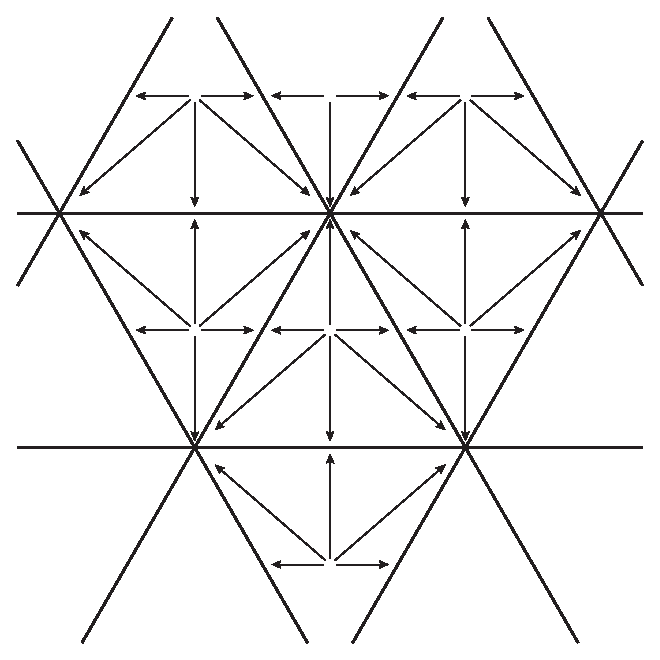
\includegraphics[scale=0.75]{fig/euler-vf-2b}
\caption{Schematic example of $V_T$ in several cells of a triangulation.}
\label{fig:vt-1}
\end{figure}

%In particular, we see that each vertex of the triangulation is a zero of the vector field and this zero acts as a sink and so has index 1. At the centre of each edge is a zero where 
In terms of the figure above, we have that each zero in the centre of a simplex $\delta^i$ is a saddle point which sends flow lines out in an $i$-dimensional hyperplane and receives flow lines from the other higher dimensional $\delta^{i+1}$ simplices. One can show that the index of the zero will be $(-1)^i$ \cite{guillemin2010differential, wrightPoincare}. Summing over all the indices gives,
\begin{align*}
\sum_{x\in V_T^{-1}(0)}\mathrm{Ind}_xV_T&=\sum_{i=1}^m\sum_{i\text{-simplices }S}\mathrm{Ind}_{c_S}V_T\\
&=\sum_i(-1)^is_i\\
&=\chi(M),
\end{align*}
where $c_S$ is the centre point of the simplex $S$.
We hence have for any vector field with a finite number of zeroes,
\[
\sum_{x\in V^{-1}(0)}\mathrm{Ind}_xV=\chi(M).
\]
It immediately follows at this point that if $M$ admits a nowhere vanishing vector field, then $\chi(M)=0$.\\

On the other hand, if $\chi(M)=0$, we know that $V_T$ has the same number of zeroes with index $+1$ as zeroes with index $-1$. We can homotope $V_T$ such that the zeroes are paired together such that every zero of index $+1$ is in a chart domain together with a single zero of index $-1$ and vice versa. 

We may then do the opposite of what the splitting lemma provides and merge the zeroes, effectively canceling each pair out, leaving us with no zeroes at all. In other words, if we take a disk around a pair of such zeroes, we have a degree 0 map on the boundary of that disk and we can extend that map onto the whole disk, leaving us with no zeroes.

This concludes the proof of the theorem.
\end{proof}
Observe that since $\chi(\mathbb{S}^n)=1+(-1)^n$ (see \cite{wrightPoincare}), we have that this also proves the statement that there exists a nowhere vanishing vector field on $\mathbb{S}^n$ if and only if $n$ is odd.

\pagebreak

\subsection{Parallelisations for $\mathbb{S}^1$, $\mathbb{S}^3$ and $\mathbb{S}^7$.}
\begin{proposition}
$\mathbb{S}^1$ is parallelisable.
\end{proposition}
\begin{proof}
By \eqref{eq:novan-vect-1}, we have $V(x,y)=(-y,x)$. If we consider the points of $\mathbb{S}^1$ via the parameterisation $(\cos\theta,\sin\theta)$, then
\[
V(\cos\theta,\sin\theta)=(-\sin\theta,\cos\theta)=\gamma'(\theta),
\] 
where $\gamma(\theta)=(\cos\theta,\sin\theta)$ is a curve on $\mathbb{S}^n$, with $\gamma'(\theta)$ tangent.

Hence, by Proposition \ref{prop:para-condn}, $V(x,y)=(-y,x)$ forms a frame for $\mathbb{S}^1$ and so we have that $\mathbb{S}^1$ is parallelisable.

\begin{figure}[h!]
\centering
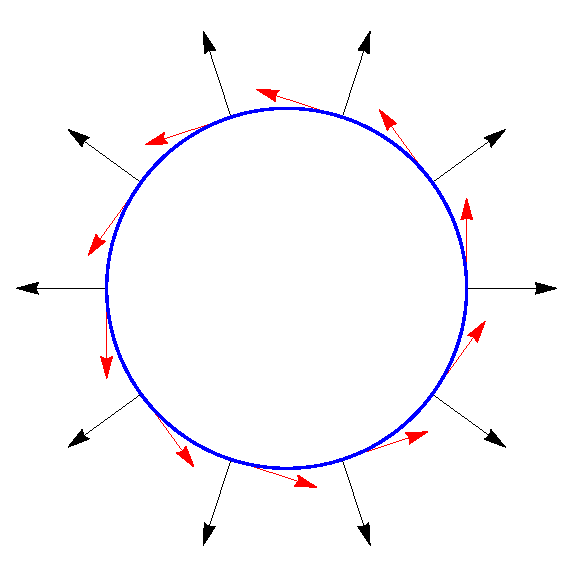
\includegraphics[scale=0.75]{fig/s1-norm-tang}
\caption{$\mathbb{S}^1$ with the vector fields $R$ (black) and $V$ (red).}
\label{fig:s1+norm+tang}
\end{figure}
\end{proof}

\begin{proposition}
$\mathbb{S}^3$ is parallelisable.
\end{proposition}
\begin{proof}
Recall the quaternion number system, $\mathbb{H}$. The quaternions are a four-dimensional, noncommutative number system. To define a product of two elements in $\mathbb{H}$ requires a choice of basis for $\mathbb{R}^4$. Elements of the basis are typically denoted by $1,i,j,k$ and elements of $\mathbb{H}$ are typically written in the form $a+bi+cj+dk$, where $i,j,k$ have the property,
\[
i^2=j^2=k^2=ijk=-1.
\]
Multiplication of $i,j,k$ can be summarised by the following diagram.

\begin{figure}[h!]
\centering
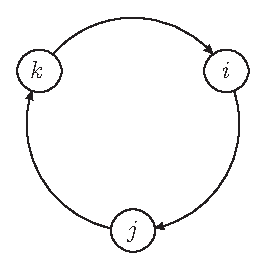
\includegraphics[scale=1]{fig/quat-mult}
\caption{Graphical representation of quaternion multiplication.}
\label{fig:quat-mul}
\end{figure}

For example, $ij=k$, $kj=-i$ and so on.

Since $\mathbb{H}$ may be identified with $\mathbb{R}^4$, we can consider $\mathbb{S}^3$ as the set of unit quaternions,
\[
\mathbb{S}^3=\left\{q=x_1+x_2i+x_3j+x_4k\in\mathbb{H}:\|q\|=1 \right\}.
\]
Considering $\mathbb{S}^3$ as the set of unit quaternions, we have that for any point $q=(x_1,x_2,x_3,x_4)\in\mathbb{S}^3$, the collection $\{iq,jq,kq\}$ forms a frame on $\mathbb{S}^3$. To show this, we compute directly as follows.
\begin{align*}
iq&=i(x_1+x_2i+x_3j+x_4k)\\
&=(ix_1+ix_2i+ix_3j+x_4k)\\
&=(x_1i+x_2i^2+x_3ij+x_4ik)\\
&=(x_1i-x_2+x_3k-x_4j)\\
&=(-x_2,x_1,-x_4,x_3)\\
jq&=j(x_1+x_2i+x_3j+x_4k)\\
&=(jx_1+jx_2i+jx_3j+jx_4k)\\
&=(x_1j+x_2ji+x_3j^2+x_4jk)\\
&=(x_1j-x_2k-x_3+x_4i)\\
&=(-x_3,x_4,x_1,-x_2)\\
kq&=k(x_1+x_2i+x_3j+x_4k)\\
&=(kx_1+kx_2i+kx_3j+kx_4k)\\
&=(x_1k+x_2ki+x_3kj+x_4k^2)\\
&=(x_1k+x_2j-x_3i-x_4)\\
&=(-x_4,-x_3,x_2,x_1)
\end{align*}
To summarise, we have the following three vector fields,
\begin{align*}
V_1&=(-x_2,x_1,-x_4,x_3),\\
V_2&=(-x_3,x_4,x_1,-x_2),\\
V_3&=(-x_4,-x_3,x_2,x_1).
\end{align*}
Note that $V_1$ is precisely the vector field one gets by applying the construction defined by \eqref{eq:novan-vect-1} to the point $q$.\\
%It remains to be shown that these are linearly independent.\\
As with the example of $\mathbb{S}^1$, consider the normal vector field to the sphere given by $N=(x_1,x_2,x_3,x_4)$. Then we have that,
\begin{align*}
\langle N,V_1\rangle&=N\cdot V_1\\
&=(x_1,x_2,x_3,x_4)\cdot (-x_2,x_1,-x_4,x_3)\\
&=-x_2x_1+x_2x_1-x_3x_4+x_4x_3\\
&=0,
\end{align*}
and similarly for $V_2$ and $V_3$. Furthermore, we observe that
\begin{align*}
\langle V_1,V_2\rangle &=V_1\cdot V_3\\
&=(-x_2,x_1,-x_4,x_3)\cdot (-x_3,x_4,x_1,-x_2)\\
&=x_2x_3+x_1x_4-x_4x_1-x_3x_2\\
&=0.
\end{align*}
Similarly, we find that $\langle V_1,V_3\rangle=\langle V_2,V_3\rangle=0$. Hence $V_1$, $V_2$ and $V_3$ are all orthogonal to the normal and hence tangent to the sphere. Furthermore we have that $V_1$, $V_2$ and $V_3$ are all linearly independent. Thus $\{V_1,V_2,V_3\}$ forms a frame on $\mathbb{S}^3$.\\
%To see that $\{V_1,V_2,V_3\}$ is a linearly independent set, consider the following. Since $\{i,j,k\}$ is a linearly independent set, this implies that $\{qi,qj,qk\}$ is a linearly independent set since $L_q:\mathbb{R}^4\to\mathbb{R}^4$ is a linear isomporhism (see the next section for details on this map). \textbf{\textcolor{red}{Bad?}}

As we will see in the next section, this type of construction generalises if we have the structure of a division algebra.
\end{proof}
\begin{proposition}
$\mathbb{S}^7$ is parallelisable.
\end{proposition}
\begin{proof}
Recall the octonions, $\mathbb{O}$. The octonions are an eight-dimensional noncommutative and nonaassociative number system. We can think of the octonions in terms of 8-tuples of real numbers, where each octonion is a real linear combination of basis octonions, $\{1,e_1,\ldots,e_7\}$. Each of the $e_i$ has the property that $e_i^2=-1$.
Multiplication of the basis octonions can be summarised by the following diagram, read in a similar manner to the analogous diagram for quaternions.\\

\begin{figure}[h!]
\centering
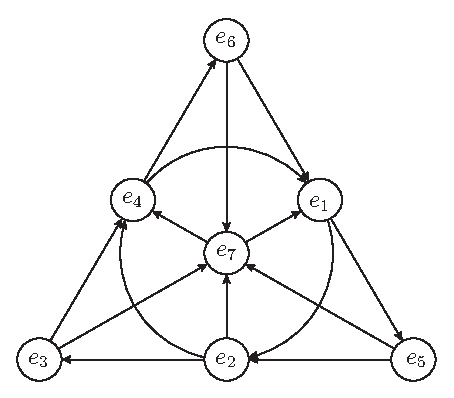
\includegraphics[scale=1]{fig/octo-mult}
\caption{Graphical representation of octonion multiplication.}
\label{fig:octo-mul}
\end{figure}

When we move to the octonions, $\mathbb{O}$, we lose the property of associativity \cite{wirthmuller_2012}. As such, $\mathbb{O}$ cannot be embedded in a matrix algebra. Instead, consider the following. Identify $\mathbb{O}$ with $\mathbb{H}^2$ and define the multiplication by,
\[
(u,v)\cdot(w,z)=(uw-vz^*,uz+vw^*).
\]
Where $q^*$ denotes the conjugate quaternion $q^*=a-bi-cj-dk$.
We have a conjugation $(u,v)\mapsto (u^*,-v)$ which provides the norm, which in turn allows one to write down the inverse of any non-zero octonion with respect to the unit $(1,0)\in\mathbb{O}$.\\

Using the same technique as in the case of $\mathbb{S}^3$, we this time consider $\mathbb{S}^7$ as the set of unit octonions,
\[
\mathbb{S}^7=\left\{q=x_0e_0+x_1e_1\cdots+x_7e_7\in\mathbb{O}:\|q\|=1 \right\},
\]
where $e_i$ are the basis octonions.
%which satisfy multiplication table.
%\begin{table}[]
%\centering
%%\caption{My caption}
%%\label{my-label}
%\begin{tabular}{l|llllllll}
%$e_ie_j$ & $e_1$ & $e_2$ &$e_3$ &$e_4$  &$e_5$  &$e_6$&$e_7$&$e_8$  \\
%\hline
%$e_1$ &$e_1$  &$e_2$  &$e_3$  &$e_4$  &$e_5$  &$e_6$&$e_7$  &$e_8$  \\
%$e_2$ &$e_2$  &$-e_1$  &$e_4$  &$-e_3$  &$e_6$&$-e_5$&$-e_8$&$e_7$  \\
%$e_3$ &$e_3$  &  &$-e_1$  &  &  &  &  &  \\
%$e_4$ &$e_4$  &  &  &$-e_1$  &  &  &  &  \\
%$e_5$ &$e_5$  &  &  &  &$-e_1$  &  &  &  \\
%$e_6$ &$e_6$  &  &  &  &  &$-e_1$  &  &  \\
%$e_7$ &$e_7$  &  &  &  &  &  &$-e_1$  &  \\
%$e_8$ &$e_8$  &  &  &  &  &  &  &$-e_1$ 
%\end{tabular}
%\end{table}

Then for any point $q=(x_0,x_1,\ldots,x_7)\in\mathbb{S}^7$, the set $\{qe_1,qe_2,\ldots,qe_7\}$ forms a frame on $\mathbb{S}^7$.
We forego writing out the entire computation here since it is simply a more tedious variation of the one carried out for $\mathbb{S}^3$.

%After the aforementioned lengthy computation, one yields the following vector fields.
\end{proof}
\begin{remark}
In view of the results presented in the next section, we note here that there was nothing stopping us from constructing the parallelisation of $\mathbb{S}^1$ using the complex numbers, just as the quaternions and octonions were used for $\mathbb{S}^3$ and $\mathbb{S}^7$ - simply take the map $z\mapsto iz$. Given the familiar setting of $\mathbb{R}^2$ and $\mathbb{S}^1$ however, there was little motivation for using this association with $\mathbb{C}$.
\end{remark}

\pagebreak
\subsection{Division Algebras}
In this section, we present some results that closely relate the existence of division algebras with the previously discussed results for sphere parallelisability.
\begin{definition}
A \textit{division algebra} is a ring in which every non-zero element has a multiplicative inverse, but in which multiplication is not necessarily commutative. For more details, see \cite{MR1415833}.
\end{definition}
\begin{theorem}
Suppose $\mathbb{R}^n$ has a division algebra structure, $m:\mathbb{R}^n\times\mathbb{R}^n\to\mathbb{R}^n$. Then $T\mathbb{S}^{n-1}$ is diffeomorphic to $\mathbb{S}^{n-1}\times\mathbb{R}^{n-1}$.
\end{theorem}
\begin{proof}
Suppose $\mathbb{R}^n$ is a division algebra. By definition of a division algebra, we have that there exists an identity element $e\in\mathbb{S}^{n-1}$ such that
\[
m(e,x)=m(x,e)=x,\,\forall x\in\mathbb{R}^n.
\]
For each point $x\in\mathbb{S}^{n-1}$, let us define the map $L_x:\mathbb{S}^{n-1}\to\mathbb{S}^{n-1}$ by,
\[
L_x(y)=\frac{m(x,y)}{\|m(x,y)\|},
\]
given some other point $y\in\mathbb{S}^{n-1}$. Since $\mathbb{R}^{n}$ is a division algebra, for each element $z\in\mathbb{S}^{n-1}$, there exists precisely one other element $y\in\mathbb{S}^{n-1}$ such that $L_x(y)=z$. Hence $L_x$ is a diffeomorphism 
%(\texttt{Is what we have thus far sufficient to conclude this I wonder?}). 
Furthermore, note that $L_x(e)=x$. Hence, we have $d(L_x)_e:T\mathbb{S}^{n-1}_e\to T\mathbb{S}^{n-1}_x$ is a linear isomorphism. Now define the diffeomorphism $f:\mathbb{S}^{n-1}\times T\mathbb{S}^{n-1}_e\to T\mathbb{S}^{n-1}$ by,
\[
f(x,v)=\left(x,d(L_x)_e(v) \right).
\]
We may now conclude that $\mathbb{S}^{n-1}\times T\mathbb{S}^{n-1}_e\cong \mathbb{S}^{n-1}\times\mathbb{R}^{n-1}$ is diffeomorphic to $T\mathbb{S}^{n-1}$.\\
%(\texttt{More detail required?}).

%\texttt{Don't quite buy/need to show}: $\mathbb{S}^{n-1}\times T\mathbb{S}^{n-1}_e\cong\mathbb{S}^{n-1}\times\mathbb{R}^{n-1}$...\\

%In addition, we note that we can always modify the multiplication map $m$ to produce an identity that fits our requirements. Specifically, choose a vector $e\in\mathbb{S}^{n-1}$. After composing the multiplication with an invertible linear map from $\mathbb{R}^n\to\mathbb{R}^n$, taking $m(e,e)$ to $e$, we may assume that $m(e,e)=e$. Let $\alpha$ be the map such that $x\mapsto m(x,e)$ and let $\beta$ be the map such that $x\mapsto m(e,x)$. Now define the new multiplication map $m'$ to be
%\[
%m'(x,y)=m\left(\alpha^{-1}(x),\beta^{-1}(x)\right).
%\]
%Observe that
%\[
%m'(x,e)=m\left(\alpha^{-1}(x),\beta^{-1}(e) \right)=m(\alpha^{-1}(x),e)=x,
%\]
%and
%\[
%m'(e,x)=x.
%\]
%Thus, we have produced a new multiplication map $m':\mathbb{R}^n\to\mathbb{R}^n$ with an identity element $e\in\mathbb{S}^{n-1}$.\\

For each point $x\in\mathbb{S}^{n-1}$, our map $L_x$ gives a linear isomorphism from $\mathbb{R}^n$ to itself. By scaling the output to have length 1, left multiplication by $x$ gives a diffeomorphism from $\mathbb{S}^{n-1}$ to itself which maps the point 1 to $x$. Taking the derivative of this diffeormorphism at the point $1$ gives a linear isomorphism from the tangent space of the sphere at the point $1$ to the tangent space at $x$. Since the point $x$ on the sphere is arbitrary, a choice of basis for the tangent space of the sphere at the point $1$ determines a trivialisation of the whole bundle of the $(n-1)$-sphere. 
\end{proof}
We also have the following alternative characterisation of the same proof which we present here for the sake of contrast.
\begin{theorem}
If $\mathbb{R}^n$ has the structure of a division algebra, then $S^{n-1}$ is parallelisable.
\end{theorem}
\begin{proof}
Choose a basis $\{e_1,\ldots,e_n\}$ of $\mathbb{R}^n$ such that $e_1=1$. Take $x\in\mathbb{S}^{n-1}$ and define
\begin{equation}
v_i(x)=xe_i-\langle x,xe_i\rangle x,\,i\geq 2.
\label{eq:vi-orig}
\end{equation}
Then we have $\langle x,v_i(x)\rangle =0$ and so $(x,v_i(x))\in T\mathbb{S}^{n-1}$, i.e. $v_i$ is a tangent vector field on $\mathbb{S}^{n-1}$. Since,
\[
\{1,e_2,\ldots,e_n\},
\]
is a linearly independent set, so is the set
\[
\{x,xe_2,\ldots,xe_n\},
\]
since we have the structure of a division algebra, meaning that $L_x$ is a linear isomorphism.

%Note that if we consider the $v_i$ as being written in the form $v_{i+1}=c_{i+1}e_i+f_{i+1}$, $v_{i+2}=c_{i+2}e_i+f_{i+2}$ for $i\geq 2$, then if $f_3=\lambda f_2$, for some scalar $\lambda$, then $e_i,e_{i+1}\in\mathrm{span}\{e_i,f_2\}$ and so on. However, since we know that the $e_i$ are linearly independent and by the above, we know that this is not the case. \texttt{TO BE FIXED LATER...}
\begin{proposition}
The vectors $v_i(x)$ form a basis for $T_x\mathbb{S}^{n-1}$.
\end{proposition}
\begin{proof}
Given a point $x\in\mathbb{S}^{n-1}$, it follows that $\{x\}^\bot=T_x\mathbb{S}^{n-1}$, i.e. the set of vectors orthogonal to $x$ on the sphere are precisely those in the tangent space at $x$.
Hence, we have the following characterisation of the vectors $v_i(x)$ in terms of a projection $\pi$ onto the orthogonal complement of $x$.
\[
v_i(x)=\pi_{\{x\}^\bot}(e_i\cdot x)=\pi_{T_x\mathbb{S}^{n-1}}(e_i\cdot x).
\]
First, note that 
\[
\dim\left(\mathrm{span}\{v_i\}_{i=2}^n\right)=n-1=\dim\left(T_x\mathbb{S}^{n-1}\right).
\]
Since the spaces under consideration are finite dimensional, it suffices to show that $\dim \pi(\mathrm{span}\{v_i\}) =n-1$.\\

Let $\{w_j\}_{j=1}^k$ with $k\leq n-1$ be a basis for $\pi(\mathrm{span}\{v_i\})$. Then $v_i=c^j_iw_j$ (where the Einstein summation convention is being used). Rearranging \eqref{eq:vi-orig} for $xe_i$, we hence have,
\begin{align*}
xe_i&=v_i+\langle x,xe_i\rangle x\\
&=c^j_iw_j+\langle x,xe_i\rangle x.
\end{align*}
Note that
\[
c^j_iw_j+\langle x,xe_i\rangle x\in\mathrm{span}\{x,w_j\},
\]
We hence have that
\begin{align*}
\mathrm{span}\{xe_i\}&\subseteq\mathrm{span}\{x,w_j\}\\
\Rightarrow n&=k+1\\
\Rightarrow k&=n-1,
\end{align*}
as was required.
\end{proof}
%We claim that it follows that the vectors $v_2(x),\ldots,v_n(x)$ are linearly independent. To see this, consider the following. Assume for a contradiction that their projections are linearly dependent. Then given $e_1,\ldots,e_{n+1}$, we can write $v_2,\ldots,v_{n+1}$ in the form
%\begin{align*}
%v_2&=c_2e_1+f_2\\
%&\,\,\,\vdots\\
%v_{n+1}&=c_{n+1}e_1+f_{n+1},
%\end{align*}
%where the $c_i$ are constants and the $f_i\in e_1^{\bot}$. Let $V=\mathrm{span}f_i$. Then $e_1,e_2,\ldots,e_{n+1}\in V\bigoplus e_1$. This would imply that the basis vectors $e_i$ are linearly dependent, a contradiction.
Hence, the vectors $v_2(x),\ldots,v_n(x)$ are linearly independent. Consequently, the map $\varphi:\mathbb{S}^{n-1}\times \mathbb{R}^{n-1}\to T\mathbb{S}^{n-1}$ defined by,
\[
\varphi(x,(t_2,\ldots,t_n))=(x,t_2v_2(x)+\cdots+t_nv_n(x)),
\]
is the isomorphism between $T\mathbb{S}^{n-1}$ and $\mathbb{S}^{n-1}\times\mathbb{R}^{n-1}$ that we seek.
\end{proof}
\pagebreak